\documentclass[a4paper]{article}
\usepackage[margin=1in]{geometry} % 设置边距,符合Word设定
\usepackage{ctex}
\usepackage{graphicx}
\usepackage{lipsum}
\usepackage{titletoc}
\usepackage{multirow}
\usepackage{fancyhdr}%设置页脚页眉需要的包
\pagestyle{fancy}
\usepackage{enumitem}
\usepackage{gbt7714}
\usepackage{subfigure}
\usepackage{threeparttable}

\title{\heiti\zihao{2} 数字经济背景下农村经济增长点研究}
\author{\songti 2000510129梁嘉铭}
\lhead{桂林电子科技大学}
\rhead{数字经济结课论文}%右边
\date{\today}
\begin{document}
\maketitle
%生成文档目录
\tableofcontents
\newpage

%构建各章节的一级小结
\section{引言}
当前,以 5G、工业互联网、人工智能、云计算、
大数据等数字技术的研发和应用为核心内容
的数字经济与数字化转型发展迅速,
给全球经济和人们生活带来了巨大的影响。\\
\begin{figure}[ht]
	\centering
	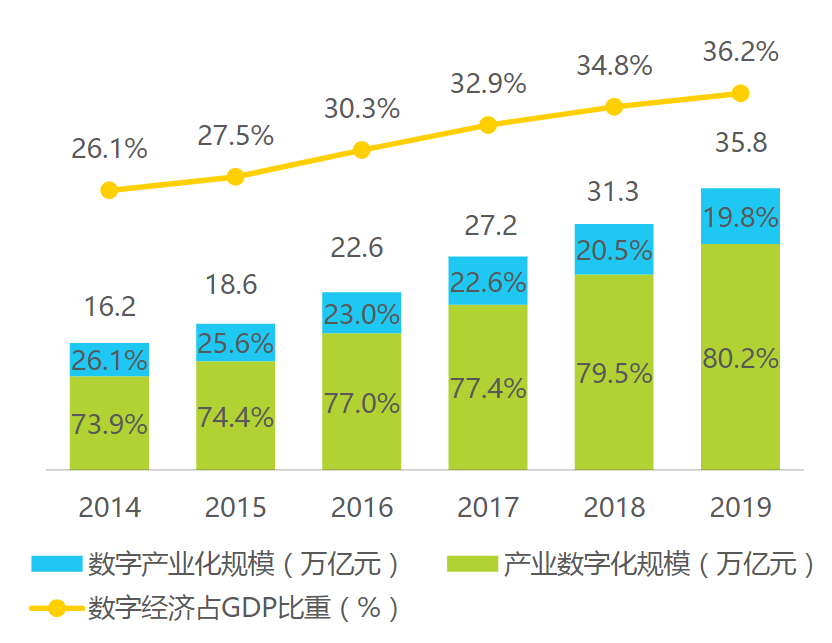
\includegraphics[scale=1]{digital.png}
	\caption{2014-2019年中国数字经济规模及增速}
	%\label{fig:label}
\end{figure}
\par
2019年我国数字经济规模达到 35.8 万亿元,
占 GDP 的比重为 36.2\%,对 GDP 增长的贡献率达 67.7\%,
成为我国经济增长的核心动力。
数字技术对各行各业的影响越来越大,
同时也会给农业农村发展带来了新的机遇,
但由于乡村也城镇资源差异,
其数字基础建设、数字技能等多方面的短板
将可能成为抑制农村数字化、减小城乡发展差距的新因素。
所以本文将系统梳理农业农村数字化转型中的特点、
关键、突出问题等内容,并提出有针对性的建议,
为未来推进农业农村数字化转型实践、
构建数字乡村提供参考借鉴
\cite{sanren}。

\section{数字农业发展特点及其内容}
数字经济作为一种新的经济形式,有着其自身的发
展特点。和传统农业相比,数字农业具有明显的互联网特征,
其利用了当今发展较快的自动化技术信息化技术来实现对
传统农业的改造。和传统的农耕产业相比,数字化农业
具有以下的内容和特点。

%构建二级小节
\subsection{农业要素数字信息化}
\begin{figure}[ht]
	\centering
	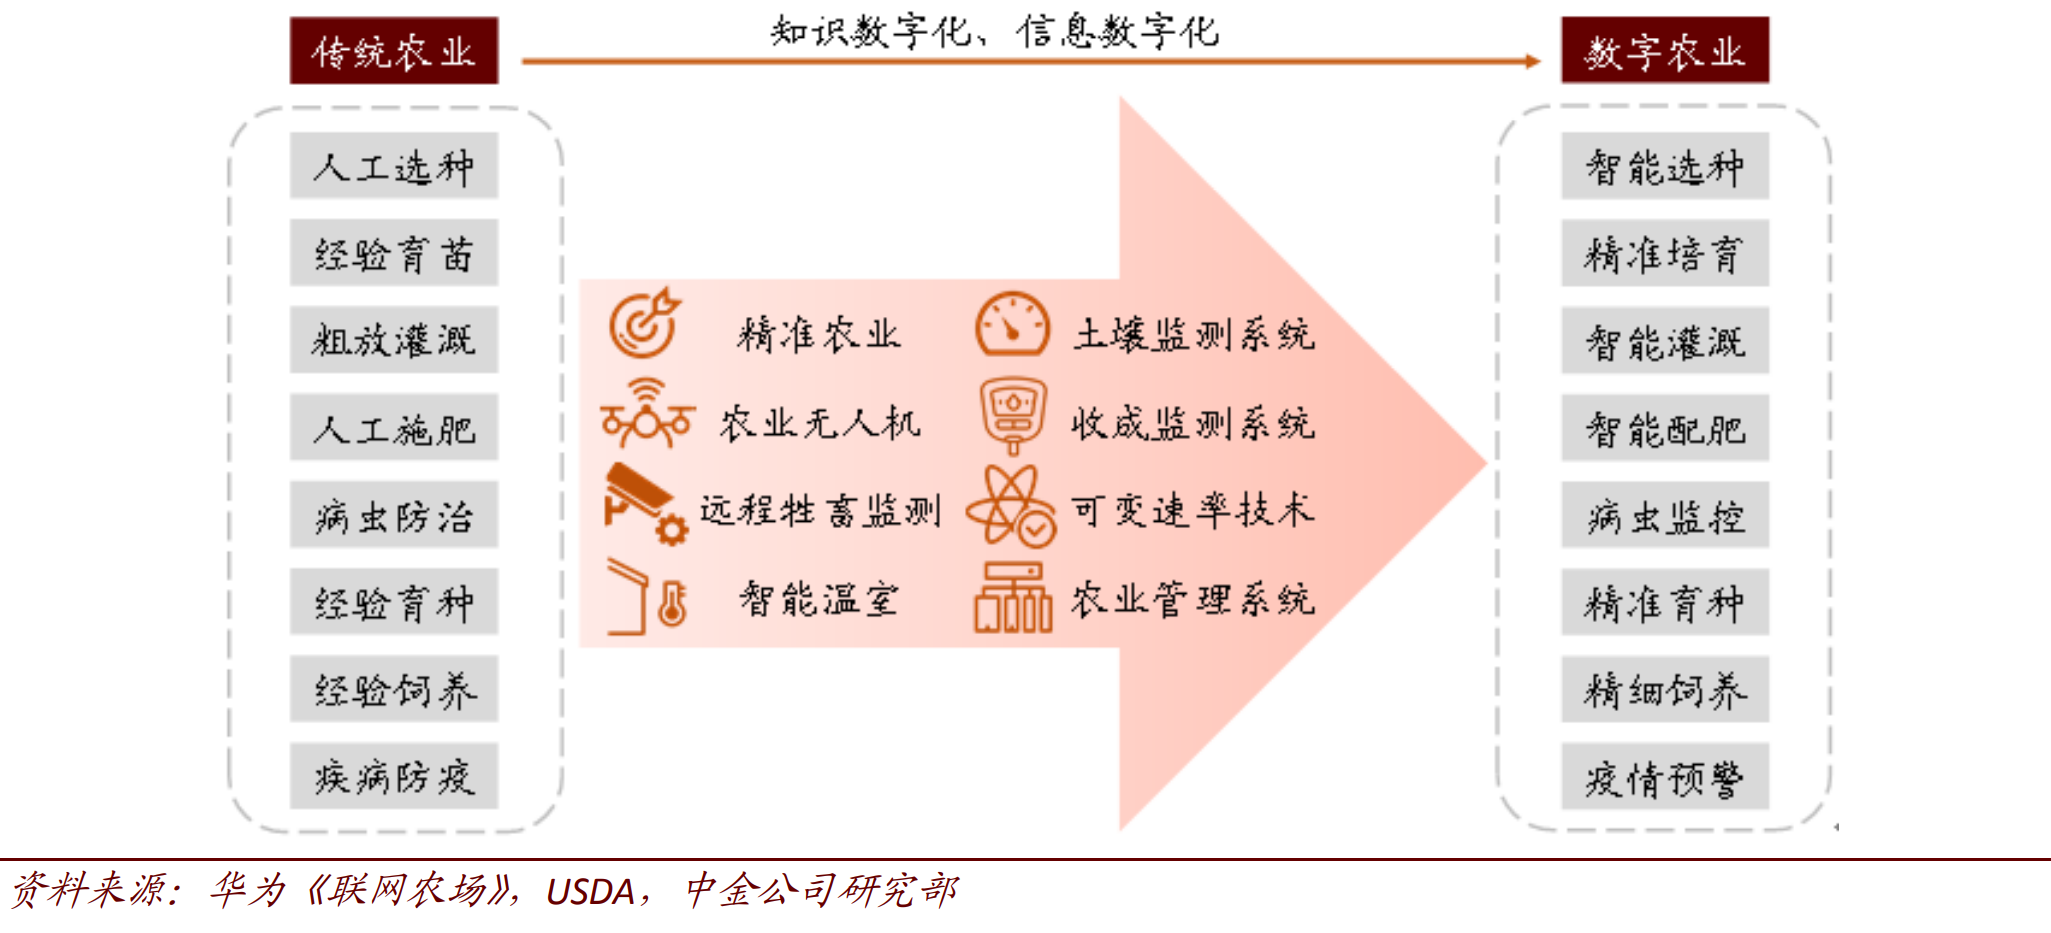
\includegraphics[scale=0.5]{longye.png}
	\caption{数字经济如何赋能农业示意图,含应用领域}
	%\label{fig:label}
\end{figure}
\par
在农业生产过程当中,有四项最重要的因素既生物、
环境、技术和社会经济的因素
\cite{中金}。
通俗的讲就是农作物在
生长以及销售的过程当中所包含的所有因素,例如农作
物生长的阳光、湿度、灌溉程度、农产品的价格、社会需求
等因素。这些因素不仅贯穿了整个农业生产的全部阶
段,同时也贯穿了农业销售的整个阶段,直接关系到农民
的投入与产出比。利用计算机技术对这些信息进行整合
概括,纵向分析可以精确的分析出农作物的生长状况以
及预期收入
\cite{zoutao}。

\subsection{农业过程的数字信息化}
随着现代农业技术的发展,如果已知农作物生产过
程中的湿度,土壤肥度,灌溉程度等要素,便可以对农作
物生长过程进行模拟,利用计算机强大的计算功能来推
算农作物的生长过程。利用这项技术,不仅可以实现对
目前农业生产活动的精准把控,还可以利用收集来的数
据进行分析研究,更好的促进农业发展
\cite{刘雨轩2019发展}。

\subsection{农业管理的数字信息化}
农业管理是农业生产过程当中比较消耗人力成本的
一项过程,主要包括农业科技管理,农业行政管理,农业
生产管理和农业企业管理。利用现代互联网技术,把农
业生产中的一些信息和要素进行集中处理。通过建立相
应的数字农业系统,将这些管理信息进行横向对比,可以
更好地对农业实施精准化管理。另外,数字信息化的农
业管理更加符合当代农业研究的要求。通过将农业管理
的信息进行数字化,可以更好的帮助专家进行农业问题
的分析,解决当前农业生产中所遇到的困扰,科学规避农
业生产活动中可能遇到的风险,以及如何更好的发展当
前农业经济等问题。可以说农业管理的信息数字化,将
农业生产与专家紧密结合在一起。在传统的农业生产过
程当中,由于农业人口基数过于庞大,无法做到专家兼顾
到每一块农田的生产,使得农业技术无法及时的与农民、
农业相结合。而农业管理的数字信息化可以说是解决了
这一问题。通过互联网技术便能够把农田的信息传到云
端,专家只需要通过对应的信息系统,便能够实现对不同
地区农业的横向比较精准分析出某块农田目前存在的问
题并给出解决措施,极大地促进了农业的发展。

\section{数字农业发展规模前景}
\textbf{全球数字农业规模千亿元级,中国处于早期发展:}
据华为《联网农场》数据,2020 年全
球数字农业市场规模约268亿美元,对应超1800亿人民币,
2015~2020年CAGR约+14.3\%。其中,我们估算 2020 年
中国数字农业规模约 34 亿美元,对应超 200 亿人民币,占全球
比例约 13\%,当前仍处于早期发展。此外,从数字农业应用领域看,
精准农业、精准牲畜饲养、收成检测、农业无人机为主,
2020 年其占全球数字农业比重合计达约 55\%。

\newpage
\begin{figure}[htbp]
	\centering
	\subfigure[全球数字农业市场规模]{
		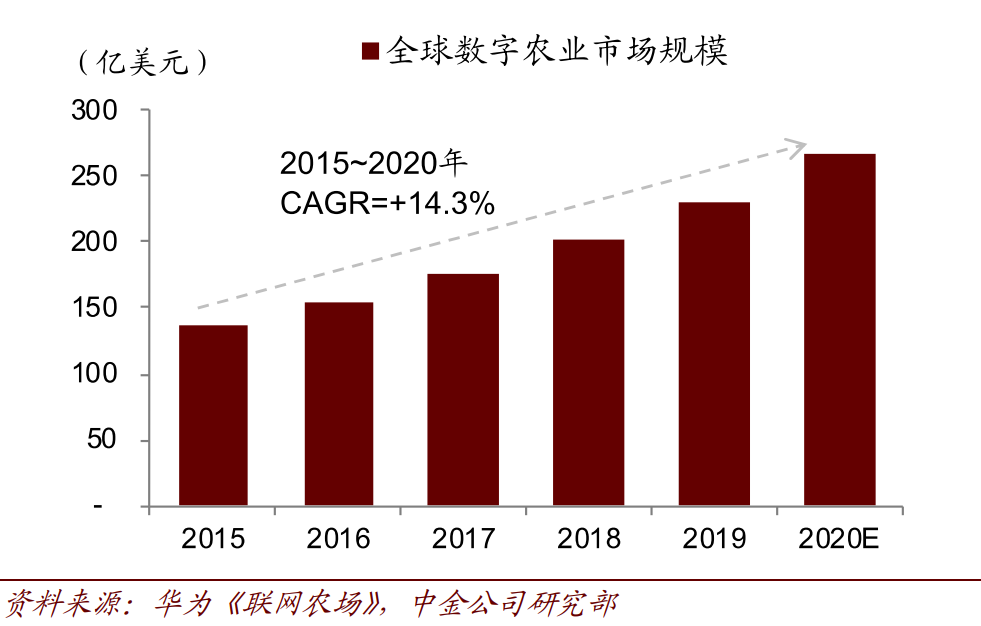
\includegraphics[width=7cm]{gimo.png}
	}
	\quad
	\subfigure[全球数字农业分布(按国别)]{
		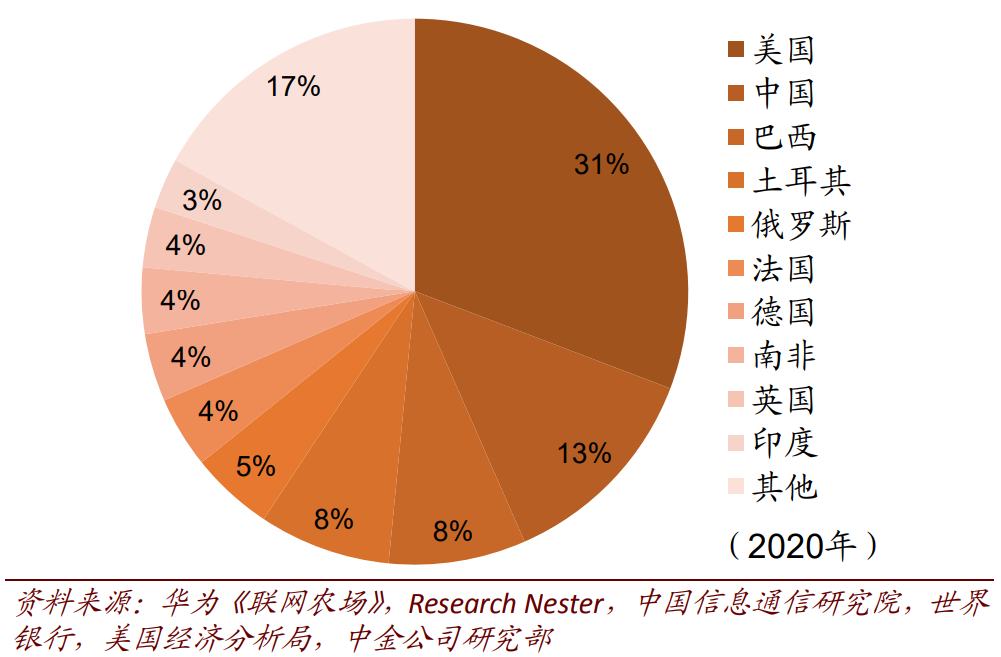
\includegraphics[width=7.3cm]{fenbu.png}
	}
\end{figure}
\begin{figure}[h]
	\centering
	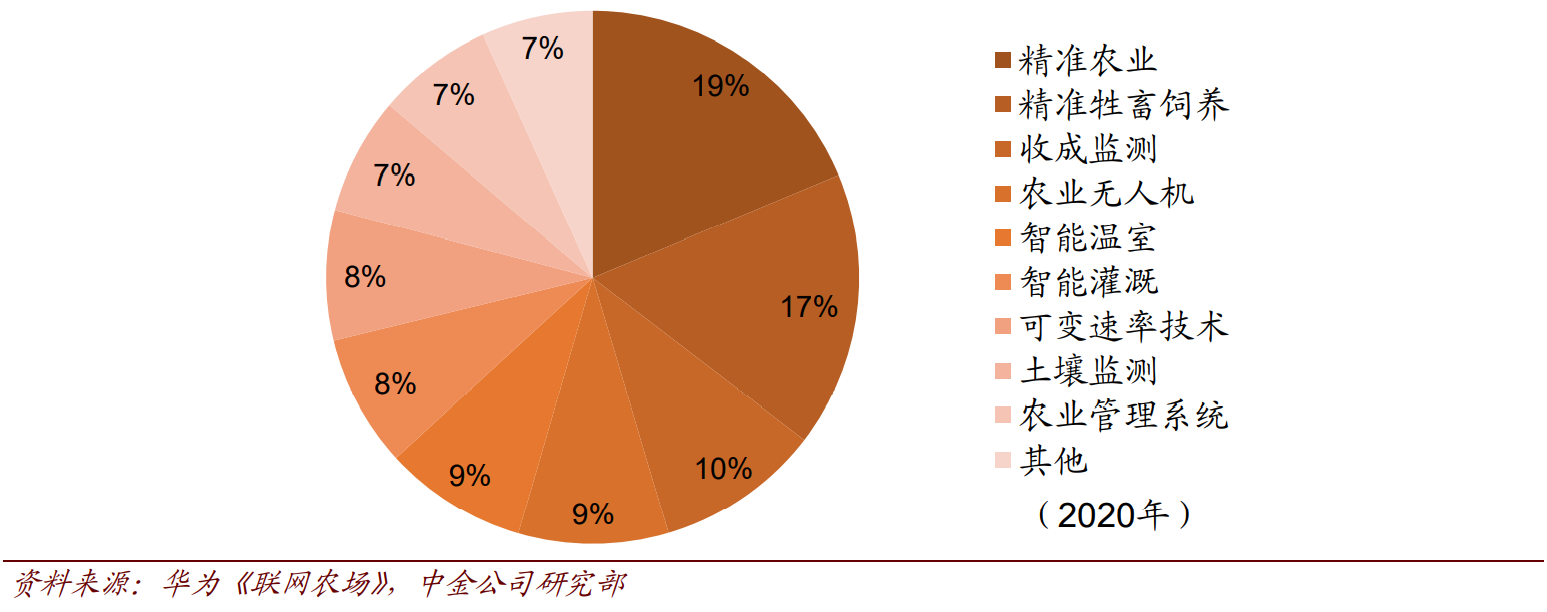
\includegraphics[scale=0.5]{caifen.png}
	\caption{全球数字农业应用领域拆分}
	%\label{fig:label}
\end{figure}
\noindent
\textbf{数字农业促进生产端革新,规模企业优势更强:}
\begin{itemize}
	\item [1)]
	      参考海外经验,美国数字农业发展较
	      早,主要通过改善生产方式以提效降本。
	      据 1965~2017 年美国农业部数据,对其估算数
	      字化令美国农业生产率提升约 9.6\%,同时各类数字化
	      技术令生产成本平均下降约 2.7\%,
	      因此数字农业应用效果集中在供给端。
	\item [2)]
	      渗透率上,随美国农场规模扩大,数字化应用越普及,
	      如 GPS 等数字农业技术,在 3800 英亩以上农场的应用率超 80\%,
	      而600 英亩以下农场仅 12\%。且在同样数字化条件下,
	      大规模农场的营业利润比中小农场高 1.1\%~2.8\%,数字农业应用
	      体现出明显的规模效应。因此我们判断数字化令大型农场竞争力提升,
	      并推动行业向头部集中。
\end{itemize}

\section{中国数字农业发展现状}
\begin{table}[!h]
	\caption{城乡互联网使用情况统计与影响}
	\resizebox{\textwidth}{!}{%
		\begin{tabular}{c|c|c|c|c|c|c|c}
			\hline
			\multicolumn{1}{l|}{\multirow{2}{*}{}}         &
			\multicolumn{2}{c|}{\multirow{2}{*}{城镇居民}} &
			\multicolumn{2}{c|}{\multirow{2}{*}{农村居民}} &
			\multirow{3}{*}{\begin{tabular}[c]{@{}c@{}}对城镇居民收入\\ 增长差距的影响\end{tabular}}     &
			\multirow{3}{*}{\begin{tabular}[c]{@{}c@{}}对农村居民收入\\ 增长差距的影响\end{tabular}}     &
			\multirow{3}{*}{\begin{tabular}[c]{@{}c@{}}当期互联网使用对弥合\\ 城乡收入增长差距的影响\end{tabular}}                                                                                                                     \\
			\multicolumn{1}{l|}{}                          & \multicolumn{2}{c|}{} & \multicolumn{2}{c|}{} &              &            &                                   \\ \cline{1-5}
			年份                                           & 不使用互联网          & 使用互联网            & 不使用互联网 & 使用互联网 &           &           &           \\ \hline
			2014                                           & 56.90\%               & 43.10\%               & 77.36\%      & 22.64\%    & 27.0\%*** & 32.6\%**  & 不显著    \\ \hline
			2016                                           & 45.48\%               & 54.52\%               & 64.60\%      & 35.40\%    & 23.7\%*** & 28.2\%*** & 4.5\%*    \\ \hline
			2018                                           & 37.66\%               & 62.34\%               & 55.81\%      & 44.19\%    & 14.8\%*** & 26.8\%*** & 12.0\%*** \\ \hline
		\end{tabular}%
	}
\end{table}
\footnotetext[1]{关于表中互联网使用情况的测算,本文使用
	中国家庭追踪调查的统计数据,并按照“该区域互联网使用率=”区域互
	联网使用人数/该区域总人数”公式计算得出。中国互联网络信息中心(CNNIC)测算了网民数量,
	截至2020 年 3 月,我国互联网普及率达到 64.5\%,农村互联网普及率仅为46.2\%,
	农村网民规模仅为城镇的39.3\%,占非网民整体的59.8\%。该网
	民数量与中国家庭追踪调查统计的互联网使用数据基本一致。*、** 和 *** 分别
	表示在 10\%、5\%和 1\%的水平上显著。
}
由表1我们可以看出,我国农业农村数字化尚处于初步探索之中,
数字化应用水平有待进一步提高,网络基础设
施等硬件设施建设水平,经营主体的数字化应
用,农民的数字技能等均存在不能满足数字化
转型要求的问题。
还因受到地区偏远、受文化教育程度不高、观念落后
等因素的影响,现在我国还有很多农村地区仍然沿用着
传统的农业经济发展模式,既无法提高农业生产效率,农
产品的品质也不理想,不少农户在农业生产中都有亏损
情况发生,虽然国家已经为促进农业经济发展而投入大
量资金、先进技术等,但是农业经济发展中的问题比较繁
杂且顽固,存在多方面阻碍,如农民在参与农业生产知识
培训时,并没有深刻理解其中内涵,所以培训内容在具体
实施过程中也没有发挥出应有的价值
\cite{李素芳}。而且还有很多
人对农业生态问题不够重视,例如焚烧秸秆容易造成生
态环境污染,但还是经常在农村地区发生,很多农户不知
如何对自己的土地资源进行合理运用,导致弄作品产品
质量不高,进而不利于后续农产品的销售工作顺利进行
\cite{digital}。

\section{推进我国农业农村数字化转型的建议}
 {\fangsong (一)加快推进农村“新基建”}
\par
补齐农村和贫困地区数字设施与服务短板
是推进农业农村数字化转型的基础。建议继续大
力推行“宽带中国”行动计划,着力实现农村通信
网络的全方位升级扩容。加快 5G、千兆光纤、卫
星 4G 等网络基础设施在部分有条件、有需求的
农村地区布设,满足农民生活、农业生产日益增
长的数字消费需求。建设更为稳定高速的农村教
育专网、医疗专网,实现所有学校、乡镇卫生院的
互联网稳定快速接入,试点推进部分县级医院
“5G+远程医疗”工程,试点推进为乡村医生配备
智能手机与专属应用的“互联网+乡村医生”工
程。 建设覆盖全部行政村的“乡村数字图书室”。
根据农村居民、新型农业经营主体的用网特征与
需求特点,开发更具个性化与针对性的资费套餐,
提升用网积极性,最大限度地发挥互联网新型基
础设施的效用。
\par
{\fangsong (二)加快推动农村电商的发展}
\par
农村电商是推进农业转型的重要途径。推进
农村电商发展再上新台阶,需要深化政府引导、
政企协作的发展模式。 鼓励地方政府购买第三
方服务,倡导企业积极承担社会责任,重点依托
互联网平台企业、农业企业和社会化服务组织的
技术、人才、平台优势,加速农村商品、服务的线
上化。鼓励支持新型农业经营主体开展数字化应
用。推动“直播带货”、“体验电商”等新一代电商务
业务模式在农村地区落地,以创新模式带动农村
非实物产品与服务发展。加大对新型农业经营主
体、快递企业等的仓储保鲜冷链物流建设支持力
度。引导社会资本参加县、乡({\fangsong 镇})、村邮政站点、
物流集散网点的数字化改造,构建以县级农村电
子商务公共服务中心、县乡级仓储物流配送中心、
村级电商服务站为基础的农村电子商务公共服
务体系,打通农村电商物流“首末一公里”。
\par
{\fangsong (三)推动互联网从消费领域向生产领域全
	面扩张}
\par
当前“互联网+”主要集中于消费领域,近几
年在农产品销售层面有长足进步,但农业的数字
化转型需要在生产领域有更大的变革。 一方面,
积极推进工业互联网、物联网在农村地区的布局
与应用,充分挖掘利用自然资源、生态资源、文化
资源、劳动力资源等,推动原生态劳作、景观农
业、休闲农业、乡村文旅等新业态发展,实现农村
地区一二三产业融合发展。 另一方面,制定农业
相关数据标准,全面开展农业机械设备、农业生
产设施的数字化改造,推动气象、水文、土壤、肥
力、育种等数据在农业生产领域的采集、流通与
应用,实现数据驱动与数据集成运用,化解农业
生产中的风险与不确定性。加大对“互联网+农业
技术”创新创业项目的支持,试点实施“新一代信
息技术与农业融合发展创新重点任务揭榜工
作”\footnote{参考《工业和信息化部办公厅关于印发〈新一代人工
	智能产业创新重点任务揭榜工作方案〉的通知》,重点以
	评选而非直接资助的方式推动相关应用技术的发展。},
推动数字技术在农业生产方面的创新与融
合应用。
\par
{\fangsong (四)构建面向农村地区的数字技能普及体系}
\par
借鉴国际电信联盟(ITU)、经济合作与发展
组织(OECD)等机构在改善农村和贫困地区居
民数字技能方面的实践经验,研发符合我国实际
情况的“数字技能政策工具包”(Digital Skills
Toolkit),着力改善农村地区居民基础数字能力,
提升农民对数字经济的认知程度。对农村地区的
学历教育、职业教育中的“电脑课”进行升级换
代,改设数字技能培养课程。对基层干部、农村教
师、乡村医生开展专门的数字技能培训。 组织实
施面向新型农业经营主体、返乡农民工、留守妇
女等群体的电子商务、网络直播、普惠金融等培
训,以及面向农村中老年群体的电脑、手机使用
技能培训。 创新培训方式,通过“家庭内部培训”
“社区志愿培训”等途径,提高培训效果。
\section{改进及建议}
文章主要用图表、数据研究了数字农业发展特点,以及提出发展数字农业
的建议,总体完整有序。但因为时间紧迫,并不能深入研究,
望海纳。
\newpage
\bibliographystyle{unsrt}%规定参考文献的样式
\begin{center}
	\bibliography{IEEEexample}  %参考文献库的名字Ref
\end{center}
\end{document}
